\documentclass[10pt,a4paper,german]{book}
\usepackage[utf8]{inputenc}
\usepackage[german]{babel}
\usepackage{graphicx}
%\usepackage{enumitem}
\author{Peter Silie}
\title{	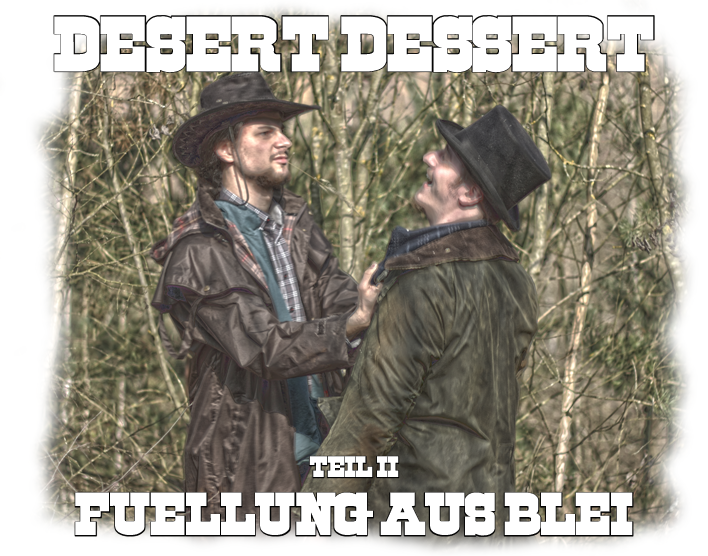
\includegraphics[scale=0.5]{titelbild.png}\\
		\vspace{1cm}
		Desert Dessert\\Teil 2\\Füllung aus Blei
		}
\date{16.04.2014}

%\setitemize{
%  fullwidth,
%  label=,
%  leftmargin=*,
%  nolistsep
%}

\begin{document}
\maketitle
\chapter{Prolog}
\section{Ende Teil 1 - Rache ist süß}
Lückenzahn Bill denkt sich in Sicherheit an einem abgelegenen Ort. Er sitzt auf einem rostigen, alten Rohr und will gerade in den erbeuteten Krapfen beissen, da wird er ihm aus der Hand geschossen. Erschrocken springt er hinter das Rohr und blickt sich langsam in der Richtung um, aus der seiner Meinung nach der Schuss gekommen ist. In der Ferne sieht man Sack'l Mac Joe auf ihn zugehen. Lückenzahn Bill springt auf das Rohr.

\begin{verse}
\textit{\glqq He! Mein Krapfen!\grqq}

Schneller Schwenk auf das Gesicht von Sack'l Mac Joe.

\textit{\glqq Und jetzt werd ich dir eine Füllung verpassen!\grqq}\\
\end{verse}

Er schießt und trifft Lückenzahn Bill, welcher daraufhin zu Boden stürzt. Fade out...
Sack'l Mac Joe nimmt sich den Krapfen aus Lückenzahns kalten, toten Händen, beisst provokativ hinein und geht dem Horizont entgegen.
Der Abspann fliegt durch das Bild.
Am Ende sieht man, dass Lückenzahn Bill nochmals in die Kamera blickt. Es bleibt offen, ob das nun ein Outtake war, ein Lustiges Ende oder ob er noch lebt.
\section{Übersicht Handlung Teil 2 - Füllung aus Blei}
\chapter{Drehbuch: Teil 2 - Füllung aus Blei}
\section{.}

\end{document}
